\documentclass[abstract=on,parskip=half,titlepage,twoside,openright]{scrreprt}

% Direct input of special characters
\usepackage[utf8]{inputenc}

% Support west european fonts / languages
\usepackage[T1]{fontenc}

% Use german translations for titles etc. (e.g. Inhaltsverzeichnis instead of Table of contents)
\usepackage[ngerman]{babel}

% Koma page style
\usepackage[automark]{scrlayer-scrpage}
\pagestyle{scrheadings}

% Bibliography
\usepackage[backend=biber,natbib=true,style=numeric-comp]{biblatex}
\addbibresource{../resources/literature.bib}

% Trademark symbol
\usepackage{textcomp}

\usepackage{listingsutf8}
\usepackage{subcaption}
\usepackage{color}

\lstdefinelanguage{wccdl}{
	morekeywords={
		as,
		by,
		class,
		classifies,
		content,
		css,
		each,
		is,
		many,
		page,
		pattern,
		recognized,
		reference,
		url,
		xpath
	},
	morestring=[s]{^^ab}{^^bb},
	sensitive=true
}

\lstdefinestyle{Xtext} {
	language = wccdl,
	basicstyle = \ttfamily\small,
	numberstyle = \footnotesize,
	showspaces = false,
	showtabs = false,
	showstringspaces = false,
	frame = single,
	tabsize = 4,
	captionpos = b,
	breaklines = true,
	numbers = left,
	breakatwhitespace = true,
	upquote=true,
	keywordstyle=\color{blue},
	stringstyle=\color{green}
}

\lstdefinestyle{pseudo} {
	language = Java,
	basicstyle = \ttfamily\small,
	numberstyle = \footnotesize,
	showspaces = false,
	showtabs = false,
	showstringspaces = false,
	frame = single,
	tabsize = 4,
	captionpos = b,
	breaklines = true,
	numbers = left,
	breakatwhitespace = true,
	upquote=true,
	keywordstyle=\color{blue},
	stringstyle=\color{green}
}

\lstset {
	basicstyle = \ttfamily\small,
	numberstyle = \footnotesize,
	showspaces = false,
	showtabs = false,
	showstringspaces = false,
	frame = none,
	tabsize = 4,
	captionpos = b,
	breaklines = true,
	numbers = none,
	breakatwhitespace = true,
	upquote=true,
	keywordstyle=\color{blue}
}

\usepackage{graphicx}
\usepackage[margin=2.5cm]{geometry}
%\usepackage{lmodern}

\usepackage[acronym]{glossaries}
\makeglossaries
\newacronym{ajax}{Ajax}{Asynchronous JavaScript and XML}
\newacronym{babw}{BaBw}{Bachelor-Studiengang Bildungswissenschaft}
\newacronym{cms}{CMS}{Content Management System}
\newacronym{css}{CSS}{Cascading Style Sheets}
\newacronym{dsl}{DSL}{domänenspezifische Sprache}
\newacronym{html}{HTML}{Hypertext Markup Language}
\newacronym{ksw}{KSW}{Kultur- und Sozialwissenschaften}
\newacronym{mvc}{MVC}{Model-View-Controller}
\newacronym{uri}{URI}{Uniform Resource Identifier}
\newacronym{url}{URL}{Uniform Resource Locator}
\newacronym{w3c}{W3C}{World Wide Web Consortium}
\newacronym{wccs}{WCCS}{Web Content Classification System}
\newacronym{wccdl}{WCCDL}{Web Content Class Definition Language}
\newacronym{www}{WWW}{World Wide Web}
\newacronym{wysiwyg}{WYSIWYG}{What You See Is What You Get}

% Support for links in pdf files
\usepackage[
	pdftex,
	hypertexnames=false,
	colorlinks=true,
	ocgcolorlinks
]{hyperref}

\hypersetup{
	unicode = {true},
	pdftitle = {Erstellung einer domänenspezifischen Sprache zur automatische Klassifizierung der Inhalte von Webseiten},
	pdfauthor = {Tim Gremplewski}
	% TODO pdfsubject = {},
	pdfkeywords = {
		{Domain Specific Languages},
		{Website Migration},
		{FernUni in Hagen}
	}
}

\titlehead{FernUniversität in Hagen\newline
Fakultät für Mathematik und Informatik\newline
Lehrgebiet Programmiersysteme\newline
Prof. Dr. Friedrich Steimann\newline
Universitätsstraße 1\newline
58097 Hagen, Deutschland\newline}
\subject{Masterarbeit}
\title{Erstellung einer domänenspezifischen Sprache zur automatischen Klassifizierung der Inhalte von Webseiten}
\author{Tim Gremplewski\thanks{tim.gremplewski@gmail.com, Martrikel-Nr: 9514244}}
\date{01. Februar 2018}

\parindent0mm

\newcommand{\editor}{Redakteur}
\newcommand{\editors}{{\editor}e}
\newcommand{\fernUni}{Fern\-Uni\-ver\-si\-tät in Hagen}
\newcommand{\imperia}{imperia CMS}
\newcommand{\resource}{Ressource}
\newcommand{\resources}{Ressourcen}
\newcommand{\wordpress}{WordPress}

\begin{document}
	\maketitle

	\begin{abstract}
		Lorem ipsum dolor sit amet, consetetur sadipscing elitr, sed diam nonumy eirmod tempor invidunt ut labore et dolore magna aliquyam erat, sed diam voluptua. At vero eos et accusam et justo duo dolores et ea rebum. Stet clita kasd gubergren, no sea takimata sanctus est Lorem ipsum dolor sit amet. Lorem ipsum dolor sit amet, consetetur sadipscing elitr, sed diam nonumy eirmod tempor invidunt ut labore et dolore magna aliquyam erat, sed diam voluptua. At vero eos et accusam et justo duo dolores et ea rebum. Stet clita kasd gubergren, no sea takimata sanctus est Lorem ipsum dolor sit amet.
	\end{abstract}

	\newpage

	\begingroup
		% No new page after table of contents
		\let\cleardoublepage\relax
		\tableofcontents
		\listoffigures
		\lstlistoflistings
	\endgroup

	\newpage

	\chapter{Modernisierung des Internetauftrittes der FernUniversität in Hagen}
    \label{chapter:FernUniRelaunch}
    Ein zeitgemäßer Internetauftritt mit aktuellen Inhalten
    ist ein wichtiger Bestandteil der Öffentlichkeitsarbeit jeder Organisation,
    da sie für viele Interessierte die erste Anlaufstelle zur Beschaffung von Informationen ist.
    
    Wichtige Gründe hierfür sind die ständige Verfügbarkeit sowie die Orts-
    und Geräteunabhängigkeit.
    Eine Webseite steht zu jeder Tageszeit zur Verfügung und kann
    dank moderner Endgeräte wie Smartphones und Tablets
    auch unterwegs aufgerufen werden.
    Für den Nutzer stellt der Internetauftritt deshalb ein Medium dar,
    das er einfach, spontan und flexibel verwenden kann.

    Wegen dieser Beliebtheit dient die Webseite neben der reinen Bereitstellung von Informationen
    auch der eigenen Werbung und Vermarktung und spielt eine wichtige Rolle im Erfolg einer Organisation.
    Zwei Eigenschaften des Webauftrittes sind laut \cite{sillence:onlineHealthSites} dabei
    entscheidend: Inhalt und Design.

    Ab einer gewissen Größe der Webseite erscheint es deshalb nachvollziehbar,
    dass zur inhaltlichen Pflege eine eigene Rolle geschaffen wird,
    die durch entsprechend ausgebildetes Personal besetzt wird.
    Ein gebräuchlicher Titel dieser Rolle ist \textit{\editor},
    der auch im Verlauf dieser Arbeit verwendet wird.

    \editors verwenden zur Pflege ihrer Inhalte üblicherweise ein \gls{cms}.
    Eine abstrakte Beschreibung solcher Systeme liefert \cite[][Seite 5,6]{barker:webCMS}:

    \begin{quote}
        A content management system (CMS) is a software package that provides
        some level of automation for the tasks required to effectively manage content.
        [...]

        A CMS allows editors to create new content, edit existing content,
        perform editorial processes on content, and ultimately make that content
        available to other people to consume it.
        [...]
    \end{quote}

    Des Weiteren beschreibt \cite[][Seite 9-12]{barker:webCMS} die Kernaufgaben eines \gls{cms}:
    \begin{enumerate}
        \item   Kontrolle der Inhalte über Rollen- und Rechtekonzepte,
                Versionierung, Abhängigkeitsmanagement, Such- und Strukturierungsmöglichkeiten
        \item   Wiederverwendung von Inhalten ermöglichen
        \item   Automatische Aggregation, Verarbeitung und Aufbereitung von Inhalten
        \item   Arbeit der \editors effizienter gestalten
    \end{enumerate}

    Wie zuvor beschrieben, ist neben dem Inhalt auch das Design,
    mit dem Inhalte präsentiert werden, relevant für den Erfolg einer Webseite.
    Die Entwicklung der Trends im Webdesign seit den frühen 1990er Jahren veranschaulicht
    \cite{work:webDesignEvolution}.
    Gezeigt wird die Entwicklung angefangen bei Seiten, die nur Text enthalten,
    über Tabellenlayouts, Flash-Applikationen bis zum Responsive Design und für
    Mobilgeräte optimierte Seiten.
    Webauftritte entwickeln sich demnach stetig weiter,
    was \cite{murphy:webDesignEvolution} an Beispielen wie der Internetseite der
    Fluggesellschaft Ryanair ebenfalls verdeutlicht.

    Folglich ist jede Organisation angehalten laufend ihre Webseite inhaltlich zu pflegen
    und ihr regelmäßig ein modernes Design zu geben.
    Andernfalls läuft sie Gefahr die Erwartungen ihrer Besucher nicht zu erfüllen,
    die sich deshalb schlecht angesprochen fühlen und womöglich zur Konkurrenz wechseln.
	\chapter{Problemanalyse}
    \label{chapter:ProblemAnalysis}
    \section{\imperia}
    \section{\wordpress}
    \section{Klassifizierung der Inhalte einer Webseite}
        %\url{http://www.fernuni-hagen.de/KSW/portale/babw/service/}

        %\begin{figure}
        %    \centering
        %    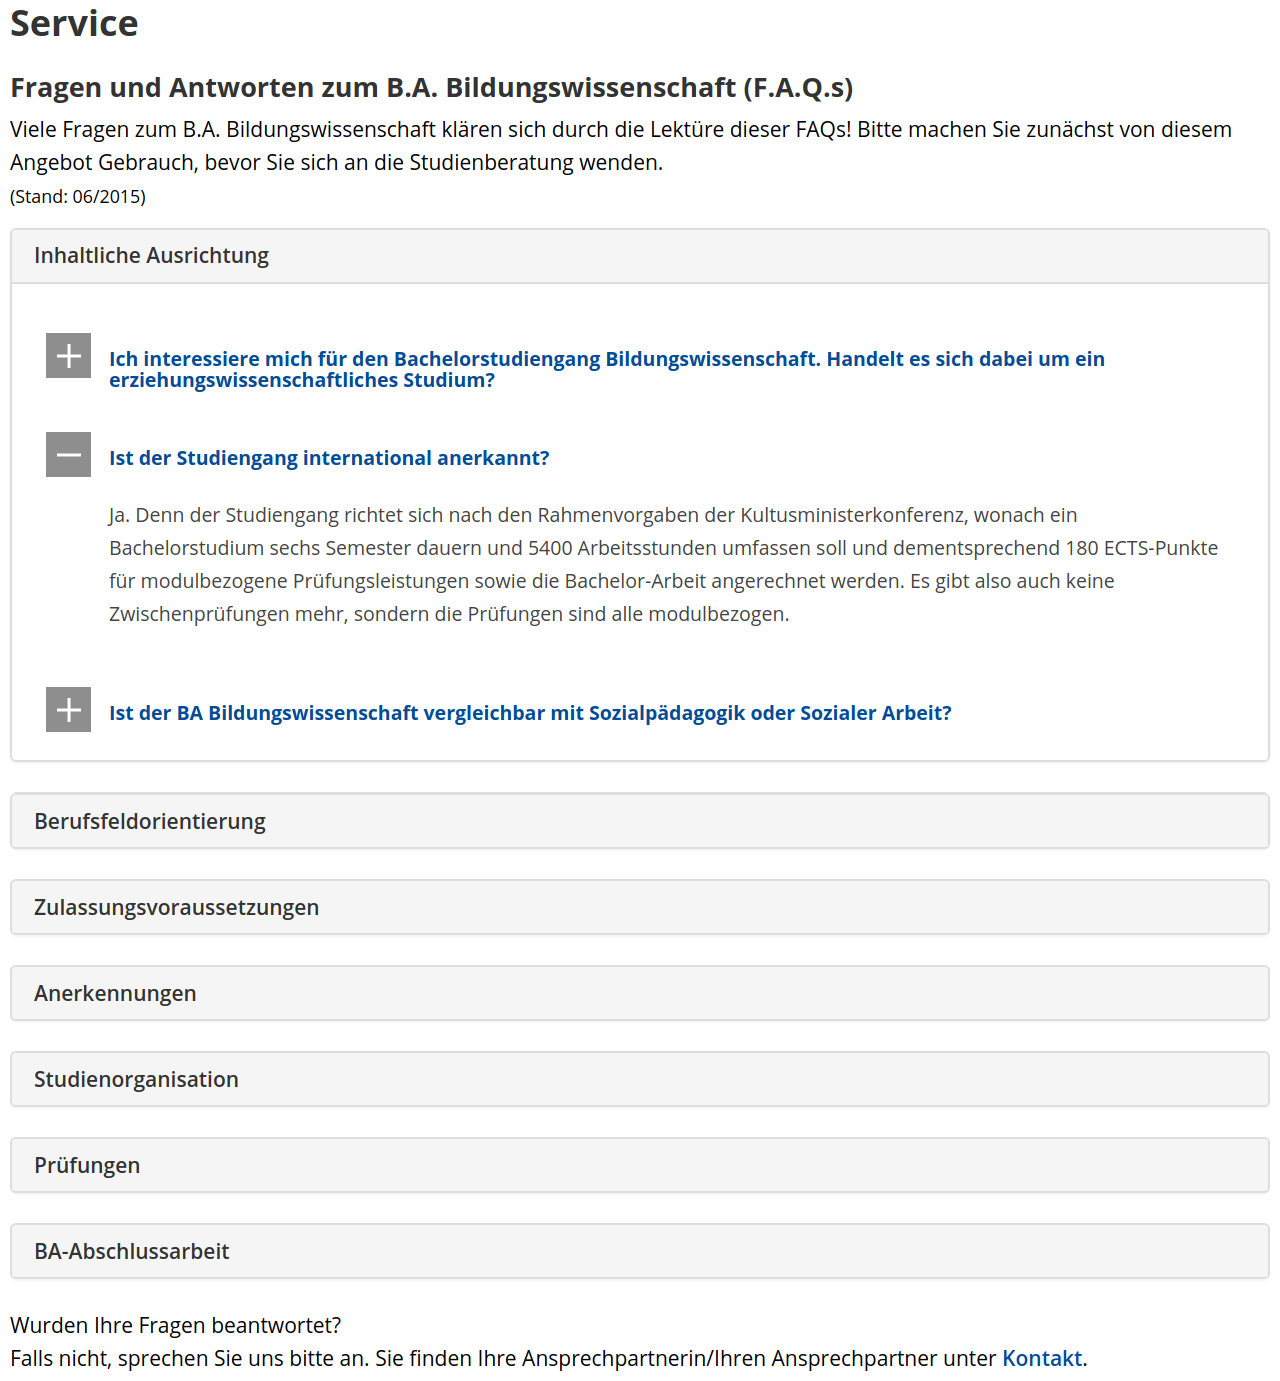
\includegraphics[width=\textwidth]{../resources/babw_service_faq.png}
        %    \caption{FAQ Seite des Studienportals B.A. Bildungswissenschaft}
        %    \label{image:BuildingBlocks}
        %\end{figure}
    
    \section{Das World Wide Web}
        Zur Lösung der beschriebenen Problemstellung ist eine genauere
        Betrachtung ihrer Domäne notwendig.
        Das Problem wird dadurch in einen größeren Kontext gesetzt,
        was zu einem besseren Verständnis und damit zur Findung
        einer geeigneten Lösung beiträgt.
        % TODO: Ref auf DDD?

        Die in diesem Fall zu betrachtende Domäne ist das "`\gls{www}"',
        welche das \gls{w3c} wie folgt definiert \cite{w3c:wwwArch}:

        \begin{quote}
            The \textit{\textbf{World Wide Web}} (\textit{\textbf{WWW}}, or simply \textit{\textbf{Web}})
            is an information space in which the items of interest, referred to as resources,
            are identified by global identifiers called Uniform Resource Identifiers (\textit{\textbf{URI}}).
        \end{quote}

        Diese Problemdomäne wird im Folgenden aus zwei Perspektiven betrachtet:
        Zunächst wird die Sicht eines Webseitenbesuchers auf das \gls{www} beschrieben.
        Anschließend stehen die konzeptionellen und technischen Grundlagen
        des \gls{www} im Vordergrund.
        Zusammen vermitteln diese Erläuterungen hinreichendes Wissen,
        um eine Lösung für die gegebene Problemstellung zu erarbeiten.

        \subsection{Das World Wide Web für Webseitenbesucher}
            Die Sicht eines Webseitenbesuchers (im Folgenden auch "`Endnutzer"' genannt)
            auf das \gls{www} ist simpel und sollte von jedem Leser nachvollzogen werden können.
            Dennoch bietet sie wichtige Einblicke.

            \paragraph*{Der Browser}
            Zugang zum \gls{www} erhält ein typischer Endnutzer über einen \textit{Browser}.
            In dessen Adresszeile trägt er einen \gls{url} ein,
            woraufhin der Browser die gewünschte Webseite lädt und anzeigt.
            Eine Webseite ist aus Sicht eines Endnutzers also eindeutig über eine
            Adresse, die allgemein "`URL"' oder "`Link"' genannt wird, gekennzeichnet.
            Der Browser dient zur Anzeige von Webseiten, wodurch er für Webseitenbesucher
            zu einem unentbehrlichen Werkzeug wird.
            Browser existieren für verschiedene Endgeräte,
            wie PCs, Smartphones und Tablets.
            Das heißt ein Webseitenbesucher ist an eine Form von Endgeräten gebunden.

            \paragraph*{Bestandteile}
            Sieht sich ein Besucher eine Webseite im Browser an,
            kann er schnell verschiedene Bestandteile ausmachen.
            Dazu zählen zunächst simple Elemente, mit denen er wenig bis gar nicht
            interagieren kann, also statischer Natur sind.
            Vertreter dieser Gruppe sind

            \begin{itemize}
                \item Texte,
                \item Bilder,
                \item Videos,
                \item Links auf andere Webseiten und
                \item Dateien, die zum Download bereitstehen.
            \end{itemize}

            Des Weiteren besitzt eine Webseite Designelemente,
            die in ihrem Aufbau oder ihrer Funktion komplexer
            als die zuvor genannten sind.
            Die Bibliothek Bootstrap\footnote{https://getbootstrap.com/}
            enthält zahlreiche solcher Komponenten.
            Beispielsweise bietet die Komponente "`Card"' die Möglichkeit
            Inhalte in komplexe Behälter einzubetten \cite{bootstrap:Cards}.
            Ein anderes Beispiel ist die Komponente "`Carousel"',
            welche der Erstellung von Diashows dient \cite{bootstrap:Carousel}.
            Letztere und viele weitere bieten dem Nutzer
            erweiterte Möglichkeiten zur Interaktion mit einer Webseite.

            Das gilt auch für Formular- oder Steuerelemente,
            die aus klassischen Applikationen bekannt sind,
            aber auch in Webseiten Anwendung finden.
            Dazu gehören unter anderem

            \begin{itemize}
                \item Textfelder,
                \item Schaltflächen,
                \item Dropdown-Listen,
                \item Checkboxen und
                \item Radiobuttons.
            \end{itemize}

            Allen Elementen ist gemein, dass ihr Aussehen sich von
            zwischen verschiedenen Webseiten unterscheiden kann.

            \paragraph{Varianten}
            Aus Sicht eines Endnutzers existieren oftmals mehrere
            Varianten derselben Webseite.
            Welche Variante er sieht hängt dabei von zwei Dimensionen ab:
            Sprache und Endgerät.

            Die heutige globalisierte und vernetzte Welt machen es oft erforderlich
            einen Internetauftritt auch auf internationele Besucher vorzubereiten.
            An erster Stelle bedeutet dies, dass Inhalte in verschiedene Sprachen
            übersetzt werden, um sie einem möglichst großen Publikum zugänglich zu machen.
            Für einen Endnutzer gibt es prinzipiell zwei Methoden,
            wie er eine Seite in seiner favorisierten Sprache anzeigen kann:

            \begin{itemize}
                \item   Die Webseite bietet ihm ein Steuerelement,
                        über das er selbst eine Sprache auswählen kann.
                \item   Die Webseite ermittelt automatisch die geeignete Sprache,
                        anhand verschiedener Parameter, die für den Besucher nicht zwangsläufig
                        offensichtlich sind.
            \end{itemize}

            Die Popularität mobiler Endgeräte wie Smartphones und Tablets
            bewegt immer mehr Betreiber von Webseiten dazu,
            verschiedene Versionen ihres Internetauftrittes anzubieten,
            die für verschiedene Geräte optimiert sind.
            Aus Sicht eines Besuchers gibt es bis zu drei geräteabhängige
            Varianten einer Webseite. Zwei für die oben genannten mobilen Geräte
            sowie eine weitere für PCs.
            Für ihn sind dabei drei Unterscheidungsmerkmale dieser Varianten offensichtlich:
            Inhalt, Design und Funktionalität.
            Ziel jeder Maßnahme ist es die Anzeigefläche,
            die ein Endgerät bietet, sinnvoll zu nutzen.
            Je kleiner ein Gerät ist, desto geringer ist diese Fläche,
            weshalb Inhalte auf kleineren Geräten weggelassen oder anderes
            dargestellt werden.
            Genauso können gewisse Funktionen einer Webseite nicht gleich
            gut sowohl auf großen PC- als auch auf kleinen Smartphone-Displays
            umgesetzt werden, ohne Anpassungen vorzunehmen.
            
            \paragraph*{Webanwendungen}
            Kapitel \ref{section:ContentManagementAndDesign} hat bereits
            kurz aufgezeigt, wie sich Webseiten stets weiterentwickeln.
            Ein wichtiger Aspekt dieser Weiterentwicklung ist aus Sicht
            eines Webseitenbenutzers, wie stark er mit ihr interagieren kann,
            was schon im Abschnitt über die Bestandteile einer Seite kurz aufgegriffen wurde.

            Angefangen bei simplen Seiten,
            die ursprünglich lediglich dazu gedacht waren Informationen
            bereitzustellen und mit anderen zu
            verlinken \cite{bernersLee:InformationManagement},
            entwickelten sich Webseiten im Laufe der Zeit weiter
            und boten immer mehr Möglichkeiten mit dem Nutzer zu interagieren
            und auf seine Aktionen zu reagieren.
            Folglich hielten immer mehr Merkmale klassischer Computeranwendungen
            Einzug in Webseiten.
            Heute stehen Webseiten klassischen Applikationen in Nichts nach,
            weshalb mit ihnen auch komplexe Anwendungen umgesetzt werden.
            Ein gutes Beispiel hierfür sind Googles Office-Anwendungen
            Docs\footnote{\url{https://www.google.com/intl/de/docs/about/}},
            Sheets\footnote{\url{https://www.google.com/intl/de/sheets/about/}},
            und Slides\footnote{\url{https://www.google.com/intl/de/slides/about/}},
            die in der Lage sind in vielen Fällen klassische Office-Anwendungen zu ersetzen.
            Aufgrund dieses besonderen Charakters ist für solche Webseiten auch der Begriff
            "`Webanwendung"' gebräuchlich.

            Im Vergleich zu herkömmlichen Anwendungen besitzen Webanwendungen zwei wichtige Vorteile.
            Solange man einen Internetzugang hat, sind sie zu jeder Zeit und von jedem Ort aus nutzbar.
            Des Weiteren können sie auf jedem Gerät ausgeführt werden,
            das einen Browser besitzt. Wie zuvor beschrieben ist dies nicht mehr ausschließlich ein PC,
            sondern auch mobile Endgeräte wie Smartphones und Tablets.

            \paragraph*{Websites}
            Der Internetauftritt einer Organisation besteht selten aus einer
            einzelnen Webseite.
            Stattdessen besteht er aus vielen Webseiten,
            die untereinander verlinkt sind und von der jede einen eigenen
            \gls{url} besitzt.
            Neben "`Internetauftritt"' hat sich der Begriff "`Website"' zur
            Referenzierung dieser Gesamtheit aller Webseiten einer Organisation
            etabliert \cite{duden:Internetauftritt, oxford:Website}.

            \paragraph*{Klassifizierung}
            Basierend auf ihrer primären Funktion lassen sich Webseiten grob klassifizieren.
            Die Bezeichnungen der resultierenden Klassen finden sich häufig im Sprachgebrauch
            von Webseitenbesucher wieder.

            Als \textit{Suchmaschinen} werden beispielsweise häufig die Seiten
            \url{https://www.google.de} und \url{https://www.bing.com/} bezeichnet.
            Andere geläufige Klassen sind:

            \begin{itemize}
                \item Online-Shops,
                \item Blogs,
                \item Homepages (Internetauftritt einer Organisation oder Privatperson),
                \item Social Networks
                \item Wikis
            \end{itemize}

            Eine weitere Kategorie sind die bereits erörterten Webanwendungen,
            also Webseiten, die bewusst als Oberflächen vob Anwendungen wahrgenommen werden.

            Viele Webseiten können unterschiedlich klassifiziert werden.
            Jede Suchmaschine und jeder Online-Shop ist gleichzeitig auch eine
            Webanwendung. Wie am Anfang dieses Abschnittes erwähnt ist für die
            Klassifizierung aus Endnutzersicht aber die primäre Funktion einer Webseite
            relevant.

        \subsection{Konzeptionelle und technische Grundlagen}
	\chapter{Lösungskonzept}
    \label{chapter:SolutionConcept}
    Dieses Kapitel erläutert ein Lösungskonzept für die in Kapitel \ref{chapter:ProblemAnalysis} beschriebene Problemstellung.
    Zentrale Elemente dieser Lösung sind ein System zur automatischen Klassifizierung der Inhalte von Webseiten
    und eine \gls{dsl} zu dessen Instrumentierung.

    XSLT kann nicht genutzt werden, da HTML kein XML ist.

    % REST-Schnittstelle für Abfrage des Contents für Klassifizierung doof,
    % weil Kontext nicht bekannt. --> Braucht man die Info überhaupt oder ist die Option aufgrund
    % anderer Anforderungen eh egal?

    \section{Klassifizierungssystem}
	\chapter{Details der Lösung}
    \label{chapter:SolutionDetails}

    \section{Klassifizierungssystem}
        % Attribute, denen URL stehen:
        % https://www.w3.org/TR/html5/links.html#links
        % https://www.w3.org/TR/html5/embedded-content-0.html#embedded-content-0

        % picture tag erst definiert in http://www.w3.org/html/wg/drafts/html/master/
	\chapter{Ergebnisse}
    \label{chapter:Findings}
    % http://www.fernuni-hagen.de/KSW/portale/babw/einstieg/lehrende-und-betreuende-im-b-a-bildungswissenschaft/
    % Seite, wo Automatisierung viel bringt
    % Telefonnummer schwierig: XPath: substring-before(substring-after(p, 'Tel.: '),'\n')
    % Dazu müsste System noch erweitert werden:
    % - Result Type ist hier anders. Es gibt kein iterateNext. D.h. nur den String auslesen
    % - Node wäre der gleiche wie Parent Node
    % - Offset müsste genau berechnet werden.
    % - Damit Annotationen funktionieren, muss Text im Parent Node stehen, nicht irgendwo anders im Dokument

    % http://www.fernuni-hagen.de/KSW/portale/lehre/bachelor-und-master-studiengaenge/
    % Da kann man gut Xpath nutzen:
    % Studiengang (als Ganzes) über h5 Selektieren
    % Name des Studienganges über XPath (self): .
    % Text zum Studiengang über XPath (nächster div): following-sibling::div[1]/p[1]
    % Hier sind inhaltliche Strukturen anders als HTML-Strukturen
    % Kann umgangen werden, da Text über einen Node angesprochen werden kann

    % http://www.fernuni-hagen.de/KSW/portale/babw/service/aktuelles/
    % Neuer Artikel über hr
    % Datum: following-sibling::p[@class='datum'][1]
    % Heading: following-sibling::h4[@class='entry-title'][1]
    % Text: Lässt sich über XPath oder CSS nicht auswählen. Man braucht "alle folgenden Nodes bis zum nächsten hr)


    % Wie viel wird auf diesen Seiten geteilt?


    % -- 3 Seitentypen in KSW --> WELCHE SIND DAS?
    % -- 1 externe Seitentypen --> WELCHE IST DAS?
    % -- Für alle Konfiguration schreiben und Klassifizierung laufen lassen
    % -- Ergebnis in Arbeit besteht aus
    % --- DSL Dateien
    % --- Klassifikation (Page Objekt)
    % --- Screenshot der Anntationen?
    % --- Screenshot der WebApp?
    % --- Wie viele Nodes werden in der Datenbank für FernUni Seiten geteilt? Schließlich sind es immer mehrere eines Typs?


    % VORGEHEN
    % - Seite aussuchen
    % - Wie ist das Modell der Seite?
    % - Konfiguration schreiben, bis es passt
    % - Wie sind die Schritte dahin?
    % - Wie sieht sie am Ende aus?
    % - Wie ist das Klassifikationsergebnis?
    % - Konfiguration auf Pendants los lassen
    % - Wie ist das Ergebnis bei diesen Seiten?
	\chapter{Diskussion der Ergebnisse}
    \label{chapter:FindingsDiscussion}

    % DSL
    % Abdeckung der Comäne (Coverage)
    % - Hängt davon ab, was Domäne ist
    % - Kann mit der Sprache jedes beliebige Struktur auf einer Webseite klassifiziert werden
    % - Siehe Formeln in Zusammenfassung
    % - Einige Spezialfälle nicht abgedeckt, siehe Ergebnisse

    % Vollständigkeit (Completeness)
    % - Sprache ist komplett
    % - Alles kann direkt in Sprache geschrieben werden.
    % - Kein D-1 Code notwendig
    % - D-1 wäre JSON. Sprache braucht das nicht.
	\chapter{Schluss}
    \label{chapter:SummaryAndOutlook}
    Zum Abschluss fasst dieses Kapitel diese Arbeit zusammen
    und zeigt einige Möglichkeiten zur Erweiterung des \glspl{wccs} auf.
    Danach zieht es ein abschließendes Fazit.

    \section{Zusammenfassung}
    Das Ziel dieser Arbeit ist die Konzeption und Entwicklung
    eines Systems zur automatischen Klassifizierung der Inhalte
    von Webseiten, was unter anderem eine domänenspezifische
    Sprache zur Instrumentierung des Systems umfasst.
    Der Titel dieses Systems ist
    "`Webpage Content Classification System"' (WCCS).
    Motiviert ist dieses Ziel durch die Modernisierung des
    Internetauftrittes der {\fernUni},
    die eine Migration von Inhalten von {\wordpress} zu
    {\imperia} beinhaltet.
    Die Herausforderung dabei ist die sehr schwache Strukturierung
    der Inhalte, wodurch sie nicht ohne Weiteres in
    Dokumente in {\imperia} transformiert werden können.
    Mithilfe des \glspl{wccs} sollen die Inhalte in einer vorbereitenden
    Maßnahme strukturiert werden, um diesem Problem zu begegnen.

    Eine wichtige Komponente des \glspl{wccs} ist eine auf Xtext basierende
    domänenspezifische Sprache namens "`Webpage Content Modeling Language"' (WCML).
    Diese erlaubt die Definition von fachlichen Seiten-, Inhalts- und
    Referenzklassen, in die Webseiten, Inhalte und Referenzen eingeordnet werden.
    Definierbare Features dieser Klassen erlauben die Schaffung feingranularer
    und hierarchischer Klassifikationen.
    Zur Einordnung von Inhalten in Klassen verwendet das System
    CSS-, XPath- und reguläre Ausdrücke, die in diesem Kontext als
    Selektoren bezeichnet werden und
    ebenfalls Teil der Klassendefinitionen sind.
    Wichtige Merkmale der \gls{wccdl} sind ihre deklarative Natur
    und ihre Lesbarkeit,
    die durch die klare Fokussierung auf eine kleine Domäne ermöglicht wird.
    Programme in dieser Sprache werden zu technischen
    Konfigurationsdateien für das Klassifizierungssystem übersetzt.

    Das \gls{wccs} klassifiziert eine Webseite auf Basis ihrer
    \gls{html}-Repräsentation und verwendet einen Webbrowser zur Auswertung der Selektoren.
    Klassifikationen können durch weitere Komponenten des \glspl{wccs}
    als Webannotationen auf der klassifizierten Webseite visualisiert werden,
    was einer Sichtung, ersten Prüfung und Durchführung kleinerer
    Korrekturen dient.
    Das \gls{wccs} speichert Klassifikationen in einer Graphdatenbank,
    wodurch die Referenzen zwischen Webseiten und anderen {\resources}
    im \gls{www} leicht abzubilden sind.
    Darüber hinaus bietet eine Graphdatenbank Vorteile bei der Modellierung,
    Speicherung und Abfrage von Klassifikationen.
    Durch die Möglichkeit Knoten des Graphen in mehreren Klassifikationen
    zu verwenden, entsteht das Potenzial weiterführende Erkenntnisse
    aus den Informationen zu ziehen.

    Anwendung hat das \gls{wccs} bei zwei Fallbeispielen der {\fernUni} gefunden,
    die gezeigt haben, dass das Konzept des Systems funktioniert,
    aber einige Sonderfälle noch nicht ausreichend abgedeckt sind.
    Ein Vergleich mit anderen Systemen hat gezeigt,
    dass die Sprache aufgrund ihrer Spezialisierung für ihren eigenen
    Anwendungsfall einige Vorteile bietet.
    Der Klassifizierungsansatz erfüllt die an ihn gestellten Anforderungen,
    ist aber weniger mächtig als komplexe Web Mining Werkzeuge.
    Ein gewisses Alleinstellungsmerkmal besitzt das \gls{wccs}
    bei der Anwendung als Werkzeug zur Prüfung der Konformität
    einer Webseite bezüglich eines individuellen inhaltlichen und strukturellen Schemas.
    \section{Ausblick}
    \label{section:endingOutlook}
    Das \gls{wccs} bietet sehr viel Potenzial um ausgebaut zu werden.

    Ein Erweiterung, von der die \gls{wccdl} profitieren würden,
    ist die Einführung eines Vererbungskonzeptes für Klassen,
    um Features und Selektoren wiederzuverwenden und die Ausdrucksstärke
    der Sprache damit zu erhöhen.
    Hierzu muss ein konsistentes Konzept für Vererbung und Polymorphie
    von Features und Selektoren geschaffen werden,
    welches sich syntaktisch gut einfügt.
    Außerdem erfordert es weitergehende semantische Prüfungen.

    Wichtig aber auch herausfordernd ist außerdem die Einbettung
    von Sprachen zur Unterstützung von CSS, XPath und regulären Ausdrücken,
    sodass die Definition von Selektoren syntaktisch und semantisch geprüft werden kann
    und ihre Formulierung durch die Entwicklungsumgebung unterstützt wird.

    Der Entwickler könnte außerdem durch ein Browser-Plugin
    deutlich bei der Formulierung von Selektoren unterstützt werden.
    Nämlich dann, wenn dieses Plugin den Browser und die Entwicklungsumgebung
    dahingehend verbindet, dass der Browser solche Elemente auf der aktuellen Seite
    hervorhebt, die durch einen bestimmten Selektor im Quelltext erfasst werden.
    Andersherum könnte der Entwickler den Browser nutzen,
    um einen Selektor eines \gls{html}-Elementes zu bestimmen und
    in die Entwicklungsumgebung zu übertragen.

    Eine Möglichkeit die beschriebenen Sonderfälle besser abzudecken ist die
    Einführung eines Skript-Selektors.
    Das heißt zur Auswahl eines HTMl-Knotens ein JavaScript Fragment ausgeführt wird,
    was prinzipiell dank der Browser-Automatisierung von Puppeteer möglich sein sollte.
    Programmatisch sollten sich auch deutlich komplexere Strukturen einfangen lassen.

    Eine weitere Maßnahme zu diesem Zweck ist die Einführung von Selektor-Ketten.
    Das heißt ein Feature wird durch eine Reihe von Selektoren
    ermittelt, wobei das Ergebnis eines Selektors als Kontext Knoten des nächsten fungiert.
    Dadurch lässt sich der Suchraum mit verschiedenen Selektor-Typen eingrenzen,
    ohne zusätzliche Features definieren zu müssen.

    In Kapitel \ref{section:discussionComparisonClassificationSystem}
    wurde das Thema maschinelles Lernen bereits kurz aufgegriffen.
    Im \gls{wccs} sind zwei Anwendungen dieser Technik denkbar:

    \begin{enumerate}
        \item   Das System wird anhand einiger Klassifikationen trainiert
                und versucht anschließend ohne exakte Vorgaben (Selektoren),
                sondern nur auf Basis des Trainings,
                neue Seiten zu erkennen und zu strukturieren.
        \item   Das System analysiert Korrekturen, die durch Nutzer durchgeführt werden
                und erzeugt Vorschläge für Änderungen in weiteren Klassifikationen.
    \end{enumerate}

    Darüber hinaus sind einige weitere kleinere Erweiterungen denkbar,
    die das Werkzeug verbessern.

    Der Nutzen des Annotator Plugins kann zum Beispiel deutlich erhöht werden,
    indem das Löschen und Anlegen von Annotationen unterstützt wird.
    Außerdem wäre es denkbar neben den vordefinierten Klassen auch
    die Angabe eigener neuer Klassen zu erlauben.

    Ein Grund der schwachen Ausdrucksstärke der Sprache ist die Notwendigkeit
    jede Klasse einzeln bekannt zu machen.

    Zur Steigerung der Ausdrucksstärke der Sprache wäre es außerdem denkbar
    einmalig genutzte Klassen ohne eigene Features nicht separat,
    sondern zusammen mit ihrer Verwendung definieren zu können.
    Das könnte zum Beispiel folgendermaßen aussehen:

    \begin{lstlisting}[style=wccdl,language=wccdl,inputencoding=utf8/latin1]
classifies myFeature as content class MyClass by css « p »
    \end{lstlisting}

    \section{Fazit}
    Die \gls{wccdl} ist eine gut lesbare und einfach zu erlernende Sprache,
    die im Sinne von domänenspezifischen Sprachen
    sich auf wenige Anwendungsfälle beschränkt
    und ihre Anforderungen dadurch gut erfüllt.
    Das \gls{wccs} als Ganzes erfüllt die gestellten Anforderungen
    trotz einiger Schwächen in gewissen Sonderfällen.

    Die Idee der Selektoren ist kein revolutionärer neuer Ansatz,
    in diesem Fall aber dennoch eine ungewöhnliche Anwendung
    zum Beispiel von CSS-Selektoren.

    Insgesamt stellt das Ergebnis der Arbeit ein funktionales System dar,
    welches im vorgesehenen Anwendungsfall gut funktioniert
    und Potenzial für weitere Arbeiten bietet.
	\appendix
	\chapter{Architektur des WCCS}
    Abbildung \ref{image:wccsExternalArchitecture} zeigt die vollständige Architektur des \glspl{wccs},
    wie sie in Kapitel \ref{section:Architecture} vorgestellt wurde.

    \begin{figure}[htb]
        \centering
        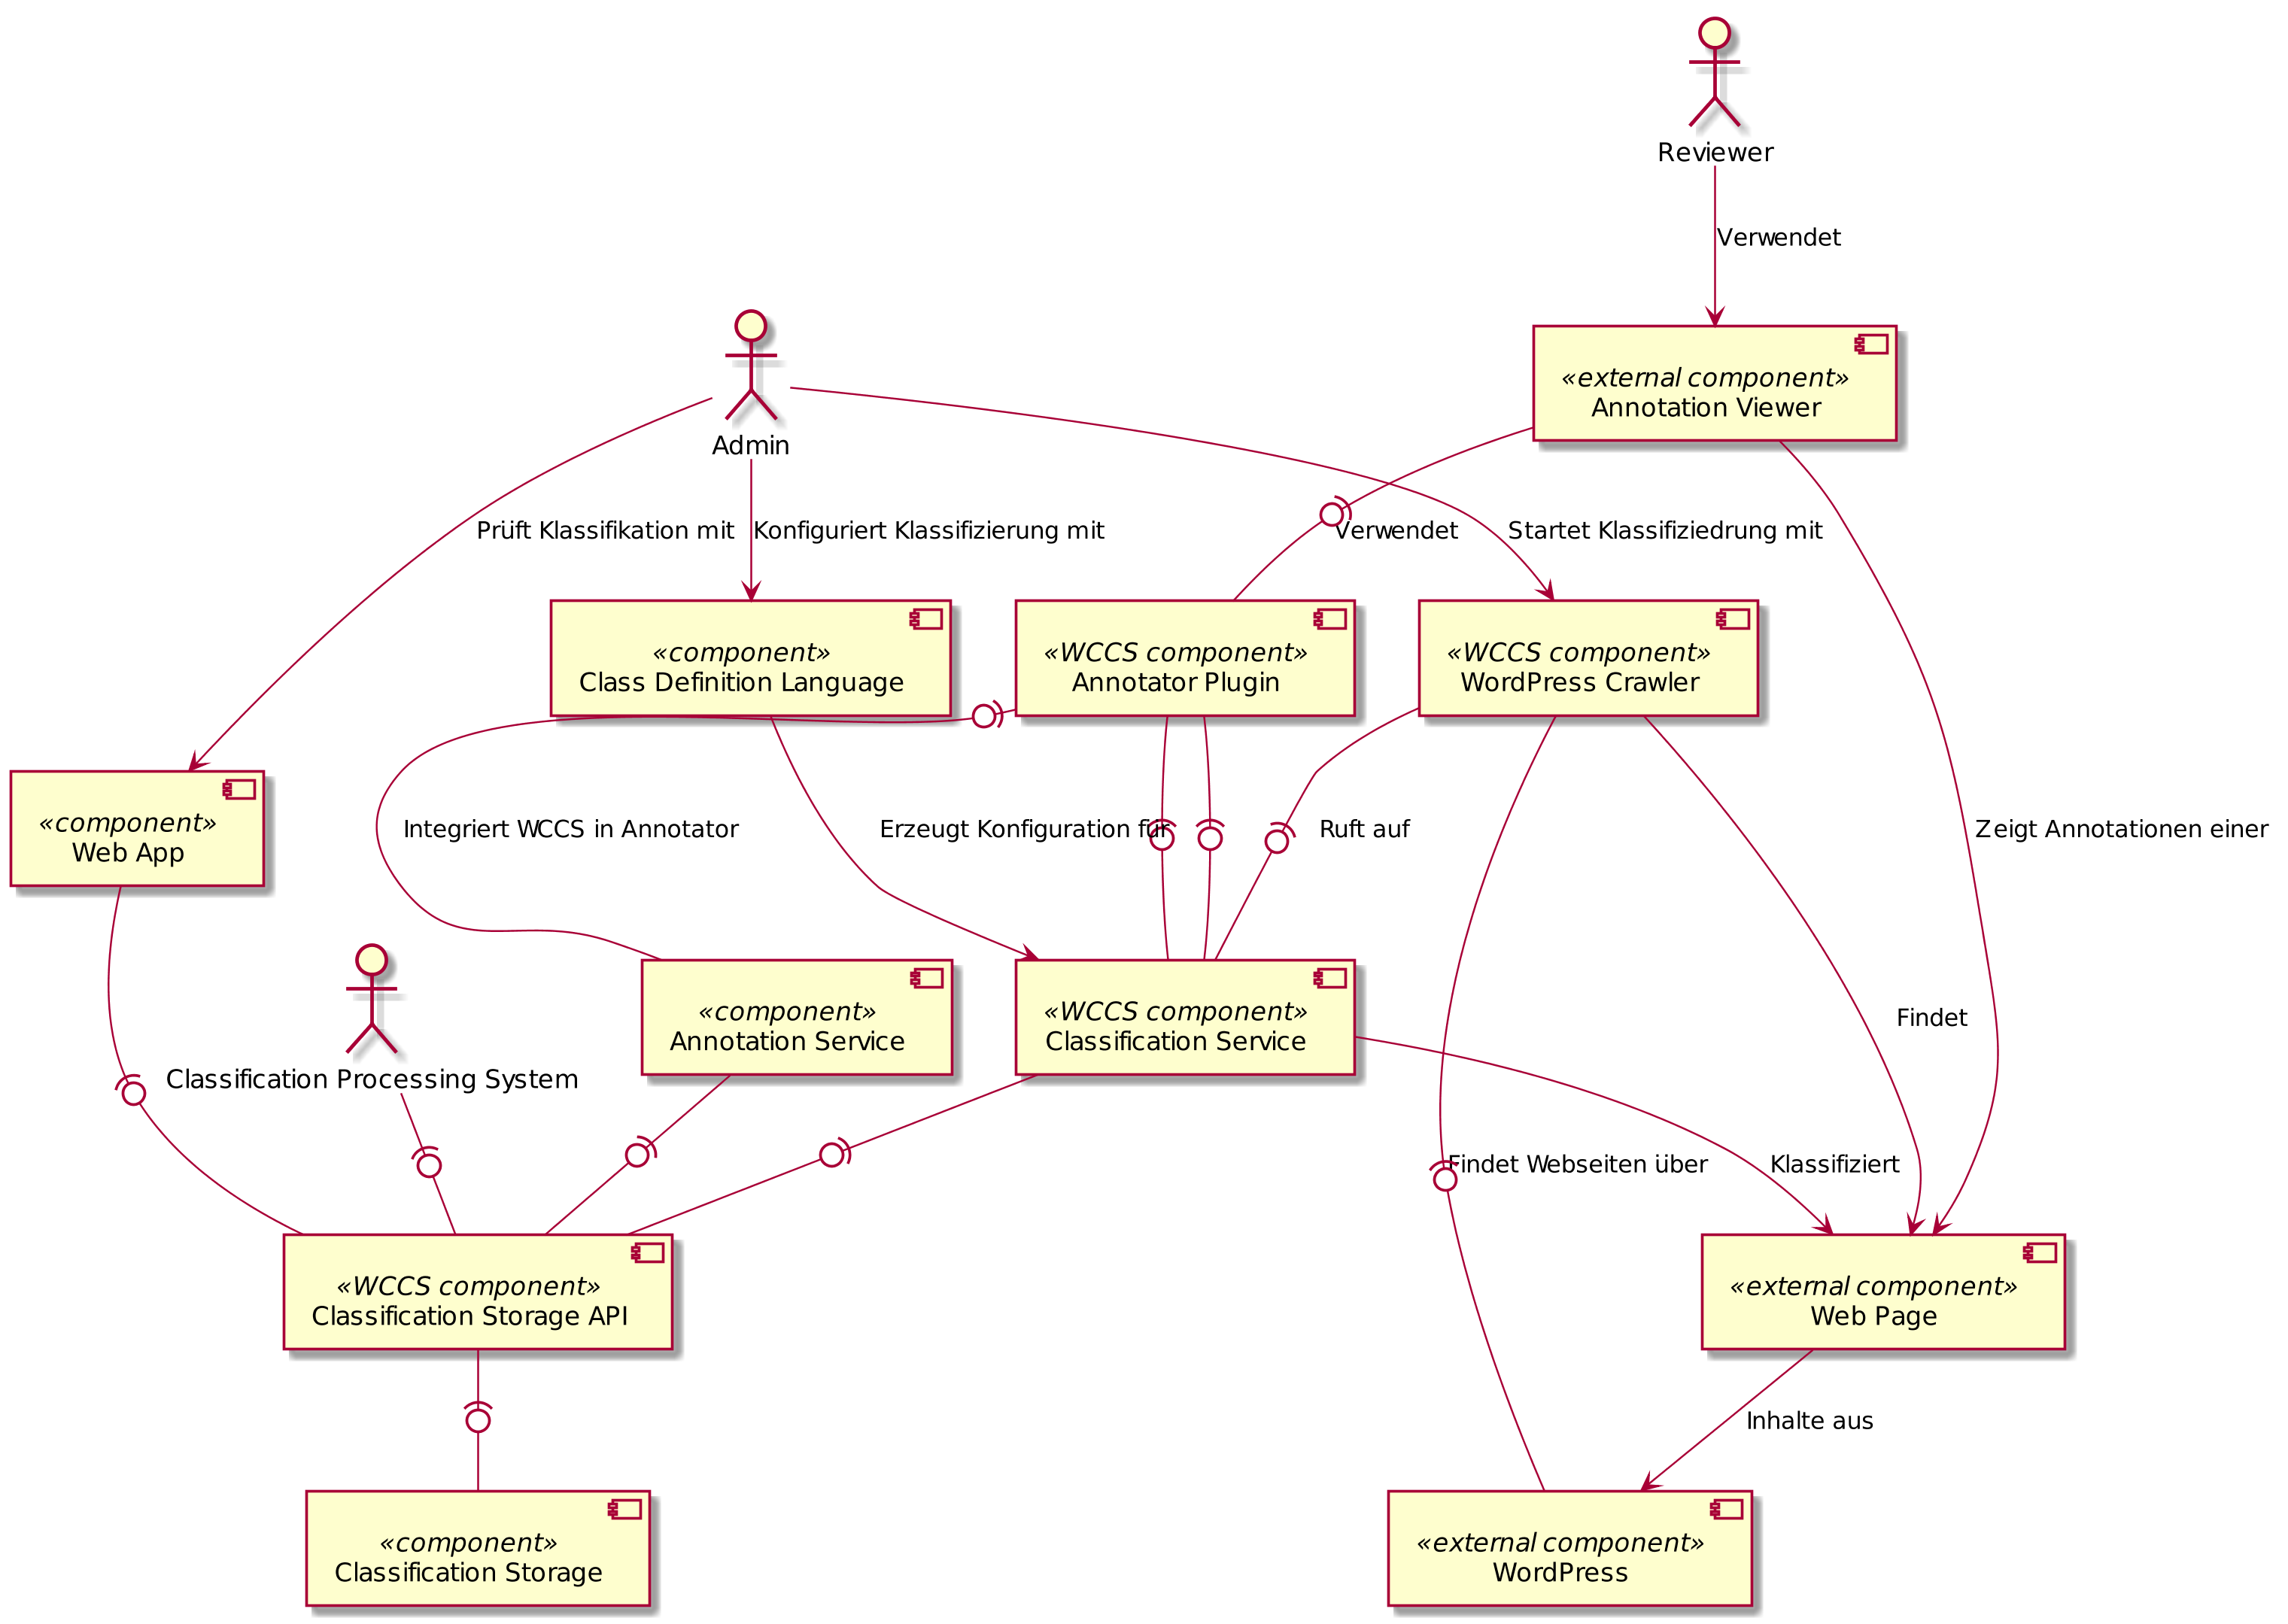
\includegraphics[width=\textwidth]{../resources/architecture/complete_architecture.png}
        \caption{Architkektur des \glspl{wccs}}
        \label{image:wccsExternalArchitecture}
    \end{figure}

\chapter{Modell der DSL}
    \begin{figure}[htb]
        \centering
        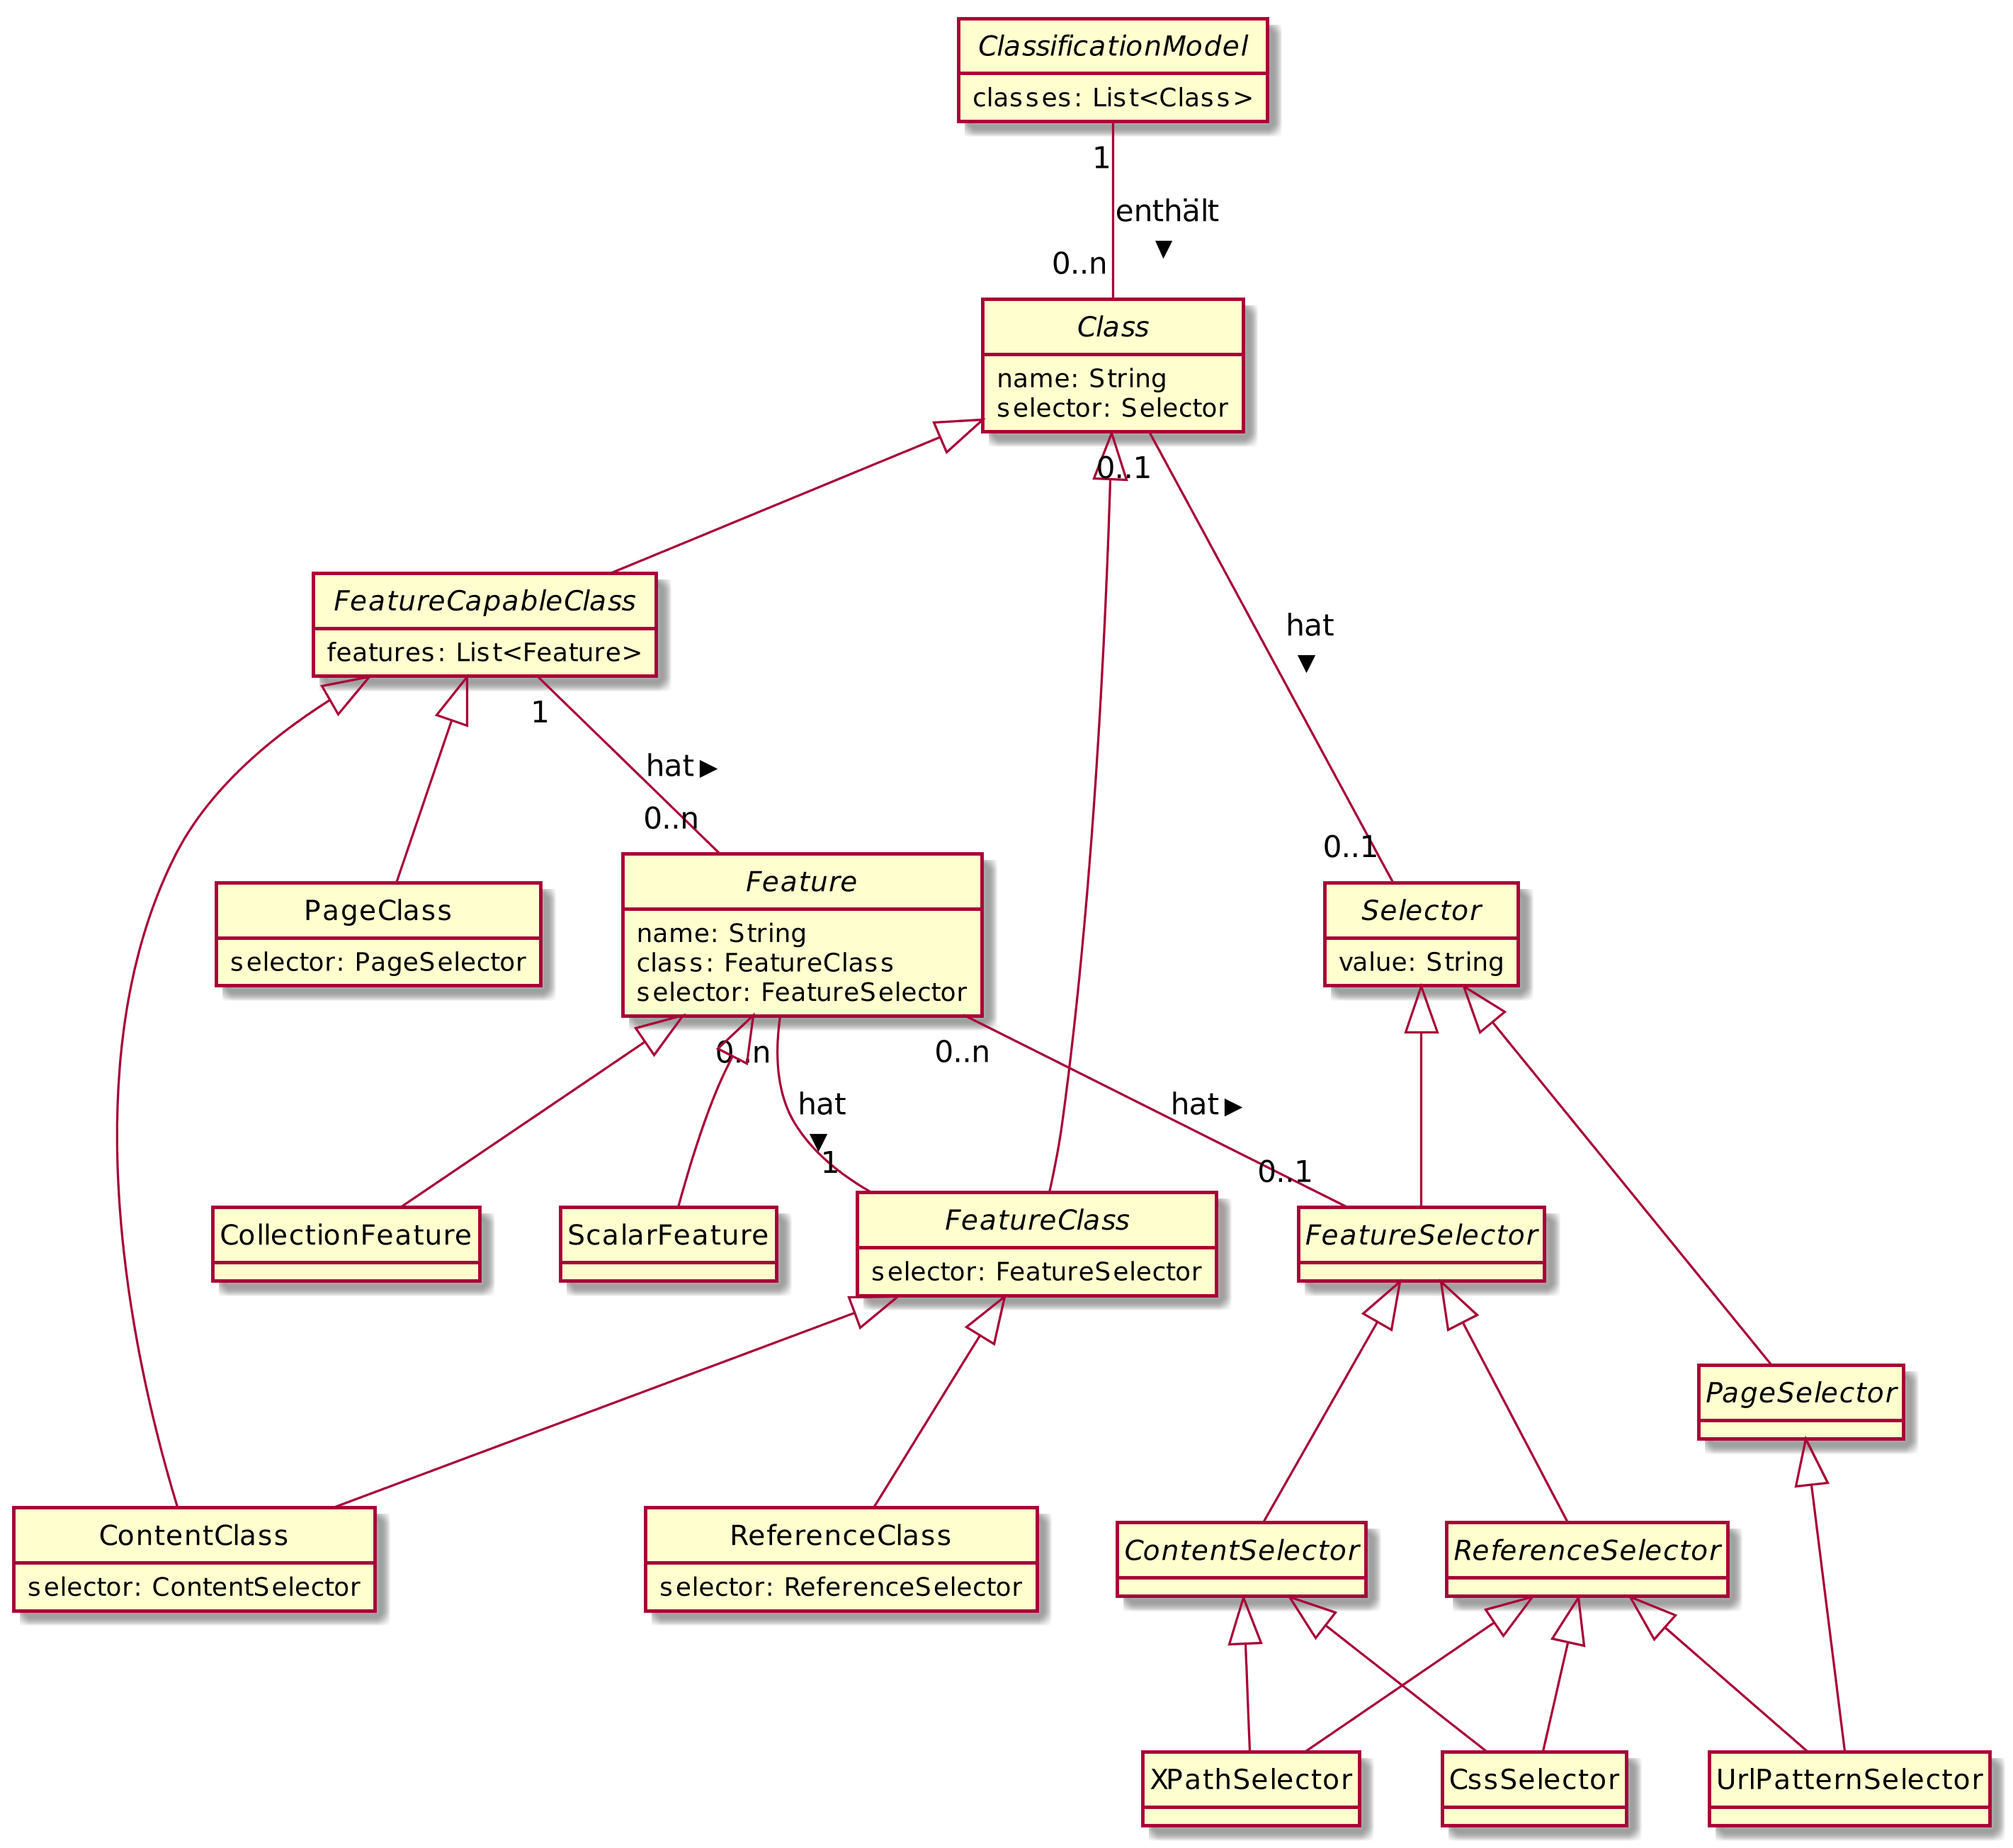
\includegraphics[width=\textwidth]{../resources/dsl/model.png}
        \caption{Modell der DSL}
        \label{image:dslCompleteModel}
    \end{figure}
	\sloppy
	\printbibliography[heading=bibintoc]
\end{document}
